% Created 2020-01-24 Fri 11:21
% Intended LaTeX compiler: pdflatex
\documentclass[pressentation,10pt,aspectratio=1610, xcolor=table]{beamer}
\usepackage[utf8]{inputenc}
\usepackage[T1]{fontenc}
\usepackage{graphicx}
\usepackage{grffile}
\usepackage{longtable}
\usepackage{wrapfig}
\usepackage{rotating}
\usepackage[normalem]{ulem}
\usepackage{amsmath}
\usepackage{textcomp}
\usepackage{amssymb}
\usepackage{capt-of}
\usepackage{hyperref}
\usepackage{fontspec,xltxtra,xunicode}
\defaultfontfeatures{Ligatures=TeX} \usepackage{appendixnumberbeamer}\usepackage{booktabs}
\usepackage[type={CC}, modifier={by-sa}, version={4.0},]{doclicense}
\usetheme{metropolis}
\usecolortheme{owl}
\author{F. Chatelain, L. Drumetz, Mauro Dalla Mura, R. Fablet, M. Fauvel, P. Tandeo}
\date{Monday 27 - Friday 31 January 2020}
\title{Data Science for Geosciences}
\subtitle{Course organization}
\metroset{progressbar=frametitle,numbering=fraction,titleformat=smallcaps,block=fill,sectionpage=simple,subsectionpage=simple}
\setbeamercovered{again covered={\opaqueness<1->{25}}}
\author[Mathieu Fauvel]{Mathieu Fauvel}
\setbeamertemplate{title page}{
\begin{minipage}[b][\paperheight]{\textwidth}
\ifx\inserttitlegraphic\@empty\else\usebeamertemplate*{title graphic}\fi
\vfill%
\ifx\inserttitle\@empty\else\usebeamertemplate*{title}\fi
\ifx\insertsubtitle\@empty\else\usebeamertemplate*{subtitle}\fi
\usebeamertemplate*{title separator}
\ifx\beamer@shortauthor\@empty\else\usebeamertemplate*{author}\fi
\ifx\insertdate\@empty\else\usebeamertemplate*{date}\fi
\ifx\insertinstitute\@empty\else\usebeamertemplate*{institute}\fi
\vspace{5mm}
\end{minipage}
}
\setbeamertemplate{footline}
{%
\leavevmode%
\hbox{\begin{beamercolorbox}[wd=.5\paperwidth,ht=2.5ex,dp=1.125ex,leftskip=.3cm]{author in head/foot}%  plus1fill,rightskip=.3cm
\usebeamerfont{author in head/foot}\insertshortauthor~(\insertshortinstitute) : \insertshorttitle
\hfill%
\end{beamercolorbox}%
\begin{beamercolorbox}[wd=.5\paperwidth,ht=2.5ex,dp=1.125ex,leftskip=.3cm,rightskip=.3cm plus1fil]{title in head/foot}%
\usebeamerfont{title in head/foot}\hfill\insertframenumber/\inserttotalframenumber\hspace{2em}
\end{beamercolorbox}}%
\vskip0pt%
}
\setbeamertemplate{blocks}[rounded][shadow=false,]
\setbeamersize{text margin left  = 0.5cm}
\setbeamersize{text margin right = 0.5cm}
\setbeamertemplate{itemize item}[square]
\setbeamertemplate{itemize subitem}[triangle]
\setbeamertemplate{itemize subsubitem}{$\star$}
\setbeamertemplate{navigation symbols}{}
\begin{document}

\maketitle

\begin{frame}[label={sec:orged1a1cd}]{Objectives}
\begin{itemize}
\item Understand the theoretical basis of 
\begin{itemize}
\item data science
\item machine learning
\item AI
\end{itemize}
\item Implement data science algorithms and models using state-of-the-art frameworks
\item Focus on applications to geosciences through dedicated projects
\end{itemize}
\end{frame}

\begin{frame}[label={sec:orgb005435}]{Organization}
\footnotesize
\begin{center}
\begin{tabular}{cp{0.15\linewidth}p{0.13\linewidth}p{0.13\linewidth}p{0.14\linewidth}p{0.13\linewidth}}
\toprule
 & Monday & Tuesday & Wednesday & Thursday & Friday\\
\midrule
09h00-12h00 & Introduction \newline Data visualization & Regression & Deep Learning & Model Selection & Project\\
\midrule
\multicolumn{6}{c}{\bf Lunch}\\
\midrule
13h30-17h30 & Project & Classification & Project & Project & Project \newline Presentation\\
\midrule
18H00-20h30 & Poster & Discussion &  &  & \\
\bottomrule
\end{tabular}
\end{center}
\normalfont
\end{frame}

\begin{frame}[label={sec:orgdc1c628}]{Scientific Team}
\begin{itemize}
\item Florent Chatelain, Grenoble INP, GIPSA-lab 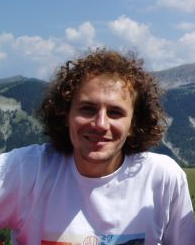
\includegraphics[width=0.08\linewidth]{pictures/florent.png}
\item Mauro Dalla-Mura, Grenoble INP, GIPSA-lab 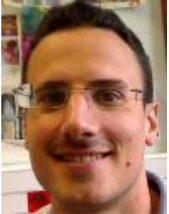
\includegraphics[width=0.08\linewidth]{pictures/mauro.png}
\item Lucas Drumetz, IMT Atlantique, Lab-STICC 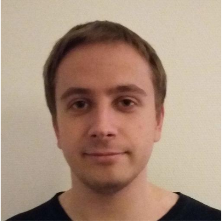
\includegraphics[width=0.08\linewidth]{pictures/lucas.png}
\item Ronan Fablet, IMT Atlantique, Lab-STICC 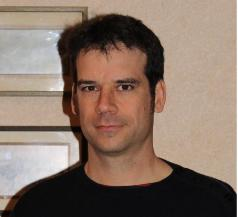
\includegraphics[width=0.08\linewidth]{pictures/ronan.jpg}
\item Mathieu Fauvel, INRAe, CESBIO
\item Pierre Tandeo, IMT Atlantique, Lab-STICC 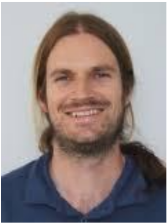
\includegraphics[width=0.08\linewidth]{pictures/pierre.png}
\end{itemize}
\end{frame}

\begin{frame}[label={sec:org779a275}]{Local Team}
\begin{itemize}
\item Mathieu Fauvel, INRAe, CESBIO 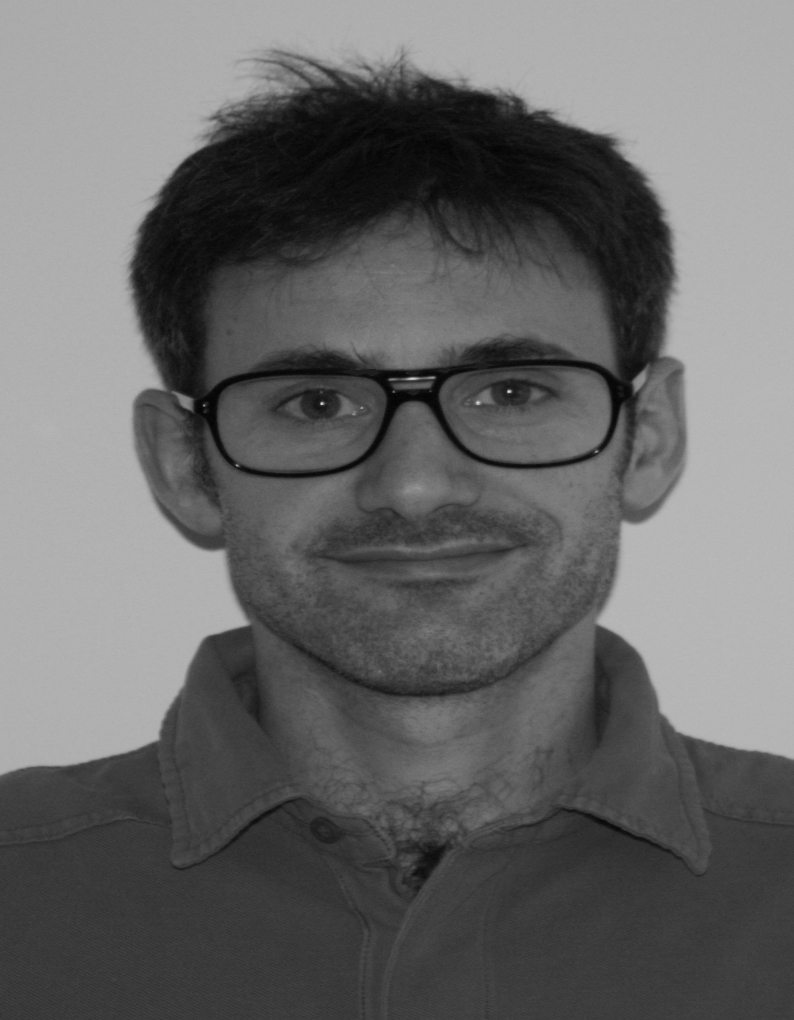
\includegraphics[width=0.08\linewidth]{pictures/mathieu.jpg}
\item Nicolas Dobigeon, Toulouse-INP, IRIT 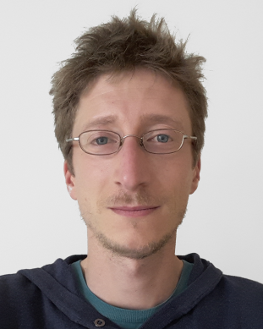
\includegraphics[width=0.08\linewidth]{pictures/nicolas.png}
\item Emilie Bastié, CESBIO
\item Delphine Maria, CESBIO
\item Anabelle Sansus, Toulouse-INP
\end{itemize}
\end{frame}

\begin{frame}[label={sec:org24d336e}]{Practical information}
\begin{itemize}
\item Course resources: Lectures, notebook, project
\begin{center}
\url{https://github.com/DataScience4Geoscience/Toulouse2020}
\end{center}
\item WIFI:
\begin{itemize}
\item EDUROAM
\item wifi-inp
\begin{itemize}
\item Login: guest\_047
\item Pass: UbWuEY7
\end{itemize}
\end{itemize}
\item Lunch:
\begin{itemize}
\item For \emph{students} only: CROUS (get your certificate, by credit card only)
\item Others: where you want/can !
\end{itemize}
\end{itemize}
\end{frame}

\begin{frame}[label={sec:org04ac605}]{Sponsors}
\begin{center}
  \begin{tabular}{ccc}
    
\includegraphics[width=0.2\linewidth]{pictures/lefe_manu.png} & 
\includegraphics[width=0.2\linewidth]{pictures/logoomp_large.jpg} &                                                                                                                          
\includegraphics[width=0.22\linewidth]{pictures/logosdu2e300dpi.jpg}\\
        
\includegraphics[width=0.2\linewidth]{pictures/logo_aniti.jpg} &     
\includegraphics[width=0.2\linewidth]{pictures/logo_avenir.png}     &     
\includegraphics[width=0.3\linewidth]{pictures/IUF_logotype_fond-transparent_off.png}
  \end{tabular}
\end{center}
\end{frame}
\end{document}